\section{拉回同态}\label{sec:pullback-homomorphisms}

\BookPairedNote
  {多项式映射是仿射簇之间保持结构的映射, 正如同态是代数对象之间保持结构的映射. 就像能在对象层面从几何走向代数, 即把 $X$ 送到 $K[X]$, 也能在映射层面从几何走向代数.}
  {粗略地说, 一族数学对象及其之间保持结构的映射, 就构成了一个\textquotedbl{}范畴\textquotedbl{}.}
\noindent 具体来说, 可以把仿射簇之间的多项式映射送到坐标环之间相应的 $K$-代数同态. 映射层面的这一转换由拉回同态给出.

\begin{Definition}{拉回同态}\leavevmode\label{def:pullback-homomorphism}
  设 $X\subseteq\mathbb{A}^{m}$ 和 $Y\subseteq\mathbb{A}^{n}$ 为仿射簇, $F:X\to Y$ 为多项式映射. $F$ 诱导的\textbf{拉回同态}为
  \[
    \begin{aligned}
      F^{*}: K[Y]&\to K[X]\\
      F^{*}(G)&=G\circ F.
    \end{aligned}
  \]
\end{Definition}

\BookPairedNoteLeft
  {注意, 拉回改变了映射方向:
   \[
     F:X\to Y\ \Longrightarrow\ F^{*}:K[Y]\to K[X].
   \]}
  {为了使拉回同态的定义有意义, 必须验证对每个 $G\in K[Y]$, 复合 $G\circ F$ 都是 $K[X]$ 的元素. 由于 $G:Y\to K$ 且 $F:X\to Y$, 根据复合的定义, $G\circ F$ 确实是一个从 $X$ 到 $K$ 的函数.}
\noindent 示意如下:
\[
  X\xrightarrow{F}Y\xrightarrow{G}K\ \Longrightarrow\ X\xrightarrow{G\circ F}K.
\]
进一步, $G\circ F$ 是多项式函数, 这是因为多项式函数的复合仍是多项式函数 (Exercise~\ref{ex:composing-with-polynomial-map}).

\begin{Example}{拉回同态}\leavevmode\label{ex:pullback-homomorphism-calculation}
  设 $X=\mathcal{V}(x_{2}-x_{1}^{2})\subseteq\mathbb{A}^{2}$, $Y=\mathcal{V}(y_{1}y_{2}-y_{3})\subseteq\mathbb{A}^{3}$. 回顾 Example~\ref{ex:parabola-map-to-hyperbolic-paraboloid} 中的多项式映射 $F:X\to Y$:
  \[
    F(a_{1},a_{2})=(a_{1}-a_{1}^{2},a_{1}+a_{2},a_{1}^{2}-a_{2}^{2}).
  \]
  考虑由 $G(b_{1},b_{2},b_{3})=b_{1}^{2}-b_{2}b_{3}$ 定义的函数 $G\in K[Y]$. 沿 $F$ 拉回, 得到多项式函数 $F^{*}(G)\in K[X]$, 定义为
  \[
    (F^{*}G)(a_{1},a_{2})=(G\circ F)(a_{1},a_{2})=(a_{1}-a_{1}^{2})^{2}-(a_{1}+a_{2})(a_{1}^{2}-a_{2}^{2}).
  \]
  类似地, 将由 $H(b_{1},b_{2},b_{3})=b_{1}+b_{2}-b_{3}$ 定义的 $H\in K[Y]$ 拉回, 得到多项式函数 $F^{*}(H)\in K[X]$, 定义为
  \[
    (F^{*}H)(a_{1},a_{2})=(H\circ F)(a_{1},a_{2})=(a_{1}-a_{1}^{2})+(a_{1}+a_{2})-(a_{1}^{2}-a_{2}^{2}).
  \]
\end{Example}

如上一例所示, 选定 $F=(F_{1},\ldots,F_{n})$ 和 $G$ 的多项式表达式后, 只需将 $F$ 和 $G$ 的多项式表达式复合, 就得到 $F^{*}(G)$ 的多项式表达式. 将这一观察展开, 设 $X\subseteq\mathbb{A}^{m}$ 和 $Y\subseteq\mathbb{A}^{n}$. 则
\[
  K[X]=\frac{K[x_{1},\ldots,x_{m}]}{\mathcal{I}(X)}
  \qquad\text{且}\qquad
  K[Y]=\frac{K[y_{1},\ldots,y_{n}]}{\mathcal{I}(Y)}.
\]
若选取多项式 $f_{1},\ldots,f_{n}\in K[x_{1},\ldots,x_{m}]$ 和 $g\in K[y_{1},\ldots,y_{n}]$, 使 $F_{i}=[f_{i}]$ 且 $G=[g]$, 则对每个 $a\in X$ 和 $b=(b_{1},\ldots,b_{n})\in Y$, 有
\[
  F(a)=(f_{1}(a),\ldots,f_{n}(a))
  \qquad\text{且}\qquad
  G(b_{1},\ldots,b_{n})=g(b_{1},\ldots,b_{n}).
\]
这蕴含
\[
  F^{*}(G)(a)=G(F(a))=g(f_{1}(a),\ldots,f_{n}(a)).
\]
因此 $F^{*}(G)=[g(f_{1},\ldots,f_{n})]$, 其中 $g(f_{1},\ldots,f_{n})\in K[x_{1},\ldots,x_{m}]$ 是将 $g$ 中的 $y_{i}$ 替换成 $f_{i}(x_{1},\ldots,x_{m})$ 所得的多项式.

\begin{Example}{再看拉回同态}\leavevmode\label{ex:pullback-by-polynomial-substitution}
  在 Example~\ref{ex:pullback-homomorphism-calculation} 的同一情形中, $F$ 的各分量函数来自多项式
  \[
    f_{1}(x_{1},x_{2})=x_{1}-x_{1}^{2},\quad f_{2}(x_{1},x_{2})=x_{1}+x_{2},\quad
    \text{以及}\quad f_{3}(x_{1},x_{2})=x_{1}^{2}-x_{2}^{2}.
  \]
  多项式函数 $G\in K[Y]$ 来自多项式
  \[
    g=y_{1}^{2}-y_{2}y_{3}.
  \]
  直接观察便可看出, 拉回函数 $F^{*}(G)$ 来自多项式
  \[
    g(f_{1},f_{2},f_{3})=(x_{1}-x_{1}^{2})^{2}-(x_{1}+x_{2})(x_{1}^{2}-x_{2}^{2}).
  \]
\end{Example}

顾名思义, 拉回同态不只是一个函数, 还是 $K$-代数同态. 下面验证这一点.

\begin{Proposition}{$F^{*}$ 是同态}\leavevmode\label{prop:pullback-is-homomorphism}
  若 $X\subseteq\mathbb{A}^{m}$ 和 $Y\subseteq\mathbb{A}^{n}$ 为仿射簇, $F:X\to Y$ 为多项式映射, 则
  \[
    F^{*}:K[Y]\to K[X]
  \]
  是 $K$-代数同态.
\end{Proposition}

\begin{Proof}
\BookPairedNote
  {要证明 $F^{*}$ 是 $K$-代数同态, 必须验证它保持加法, 乘法和数乘. 我们正式证明第一个性质, 把其余两个留给 Exercise~\ref{ex:pullback-preserves-multiplications}.}
  {有高等线性代数基础的读者也许会看出, 拉回同态是线性映射的对偶映射的推广; 见 Exercise~\ref{ex:pullback-restricts-to-dual-map}.}
\noindent 为说明 $F^{*}$ 保持加法, 设 $G_{1},G_{2}\in K[Y]$ 为两个多项式函数. 在任意 $a\in X$ 处对 $F^{*}(G_{1}+G_{2})$ 求值, 得到
\[
  \begin{aligned}
    \bigl(F^{*}(G_{1}+G_{2})\bigr)(a)&=\bigl((G_{1}+G_{2})\circ F\bigr)(a)
       &&\text{(拉回的定义)}\\
    &=(G_{1}+G_{2})(F(a)) &&\text{(复合的定义)}\\
    &=G_{1}(F(a))+G_{2}(F(a)) &&\text{($K[Y]$ 中 $+$ 的定义)}\\
    &=(G_{1}\circ F)(a)+(G_{2}\circ F)(a) &&\text{(复合的定义)}\\
    &=\bigl((G_{1}\circ F)+(G_{2}\circ F)\bigr)(a) &&\text{($K[X]$ 中 $+$ 的定义)}\\
    &=(F^{*}G_{1}+F^{*}G_{2})(a) &&\text{(拉回的定义)}.
  \end{aligned}
\]
所以 $F^{*}(G_{1}+G_{2})=F^{*}G_{1}+F^{*}G_{2}$, 这就验证了 $F^{*}$ 保持加法.
\end{Proof}

回顾一下, 我们引入拉回同态, 是为了取得判定两个仿射簇是否同构的代数工具. 由于在任何范畴中, \textquotedbl{}同构\textquotedbl{}的定义都要求验证两个态射的复合等于恒等映射, 为实现这一目标, 首先要证明拉回与复合及恒等函数相容.

\begin{Proposition}{拉回保持复合与恒等映射}\leavevmode\label{prop:pullback-preserves-compositions-and-identity}
  设 $X\subseteq\mathbb{A}^{\ell}$, $Y\subseteq\mathbb{A}^{m}$ 和 $Z\subseteq\mathbb{A}^{n}$ 为仿射簇.
  \begin{enumerate}
    \item 若 $F:X\to Y$ 和 $G:Y\to Z$ 为多项式映射, 则
      \[
        (G\circ F)^{*}=F^{*}\circ G^{*}.
      \]
    \item 恒等函数的拉回是恒等函数:
      \[
        (\operatorname{id}_{X})^{*}=\operatorname{id}_{K[X]}.
      \]
  \end{enumerate}
\end{Proposition}

\begin{Proof}
\BookPairedNote
  {为证明第一条, 设 $H\in K[Z]$. 利用复合的结合律, 计算如下.}
  {在范畴论中, 拉回的这些性质称为\textquotedbl{}函子性\textquotedbl{}.}
\[
  (G\circ F)^{*}(H)=H\circ(G\circ F)=(H\circ G)\circ F
    =F^{*}(H\circ G)=F^{*}(G^{*}(H)),
\]
这说明 $(G\circ F)^{*}=F^{*}\circ G^{*}$. 对于第二条, 设 $H\in K[X]$. 则
\[
  (\operatorname{id}_{X})^{*}(H)=H\circ\operatorname{id}_{X}=H,
\]
所以 $(\operatorname{id}_{X})^{*}$ 确实是 $K[X]$ 上的恒等函数.
\end{Proof}

现在可以实现用坐标环判定仿射簇是否同构的目标了.

\begin{Corollary}{同构的拉回仍是同构}\leavevmode\label{cor:pullback-of-isomorphism}
  设 $X\subseteq\mathbb{A}^{m}$ 和 $Y\subseteq\mathbb{A}^{n}$ 为仿射簇. 若 $F:X\to Y$ 是同构, 则 $F^{*}:K[Y]\to K[X]$ 是同构.
\end{Corollary}

\begin{Proof}
  设 $F:X\to Y$ 为同构, 其逆为 $F^{-1}:Y\to X$. 为证明 $F^{*}$ 是同构, 只需证明 $F^{*}$ 与 $(F^{-1})^{*}$ 互为逆映射. 利用 Proposition~\ref{prop:pullback-preserves-compositions-and-identity} 验证如下:
  \[
    F^{*}\circ(F^{-1})^{*}=(F^{-1}\circ F)^{*}=(\operatorname{id}_{X})^{*}=\operatorname{id}_{K[X]}
  \]
  以及
  \[
    (F^{-1})^{*}\circ F^{*}=(F\circ F^{-1})^{*}=(\operatorname{id}_{Y})^{*}=\operatorname{id}_{K[Y]}.
  \]
\end{Proof}

Corollary~\ref{cor:pullback-of-isomorphism} 的逆命题也成立, 但证明还需要一些工具, 因此留到下一节再讨论. 现在先看几个应用上述结果的例子.

\begin{Example}{$\mathcal{V}(xy)\not\cong\mathbb{A}^{1}$}\leavevmode\label{ex:crossing-lines-not-isomorphic-to-line}
  考虑仿射簇 $X=\mathcal{V}(xy)\subseteq\mathbb{A}^{2}$. 我们来证明 $X$ 不同构于 $\mathbb{A}^{1}$. 直观上, 从\hyperref[fig:crossing-lines-vs-line]{下图}画出的两个簇应当不难看出这一点. 具体来说, $X$ 由相交于一点的两条仿射直线组成, 看起来当然与一条仿射直线很不同.
  \par\smallskip
  {\centering\phantomsection\label{fig:crossing-lines-vs-line}%
  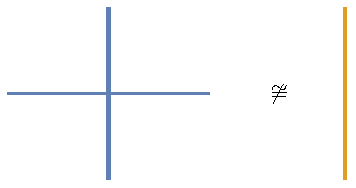
\includegraphics[width=.53\linewidth]{figures/crossing-lines-vs-line.pdf}\par}
  \smallskip
  为把这一直觉说准确, 注意 $X=\mathcal{V}(x)\cup\mathcal{V}(y)$ 是可约仿射簇. 因此 $\mathcal{I}(X)$ 不是素理想, 从而
  \[
    K[X]=\frac{K[x,y]}{\mathcal{I}(X)}
  \]
  不是整环. 由于 $K[\mathbb{A}^{1}]=K[z]$ 是一元多项式环, 它是整环. 因而, 由于同构保持\textquotedbl{}是整环\textquotedbl{}这一性质, 可知 $K[X]\not\cong K[\mathbb{A}^{1}]$, 由 Corollary~\ref{cor:pullback-of-isomorphism} 的逆否命题可得 $X\not\cong\mathbb{A}^{1}$.
\end{Example}

上一例很容易推广: 若一个仿射簇不可约而另一个可约, 则它们不可能同构, 因为其中一个的坐标环是整环, 而另一个的不是. 相比之下, 下一例说明怎样证明两个\emph{不可约}仿射簇不同构, 这可能更棘手. 这个例子还完成了我们在 Example~\ref{ex:cusp-bijective-map-not-isomorphism} 中开始的讨论, 即仿射簇之间的双射多项式映射不一定是同构.

\begin{Example}{$\mathcal{V}(x^{2}-y^{3})\not\cong\mathbb{A}^{1}$}\leavevmode\label{ex:cusp-not-isomorphic-to-line}
  与 Example~\ref{ex:cusp-bijective-map-not-isomorphism} 一样, 设 $X=\mathcal{V}(x^{2}-y^{3})\subseteq\mathbb{A}^{2}$. 为说明由 $f(a)=(a^{3},a^{2})$ 定义的多项式双射 $F:\mathbb{A}^{1}\to X$ 没有多项式逆映射, 我们证明 $X\not\cong\mathbb{A}^{1}$. 为此, 分析这两个簇的坐标环. 由于 $x^{2}-y^{3}$ 不可约, $X$ 的消没理想为
  \[
    \mathcal{I}(X)=\langle x^{2}-y^{3}\rangle.
  \]
  因此
  \[
    K[X]=\frac{K[x,y]}{\langle x^{2}-y^{3}\rangle}.
  \]
  要证明 $X\not\cong\mathbb{A}^{1}$, 只需找到一元多项式环 $K[\mathbb{A}^{1}]=K[z]$ 具有而 $K[X]$ 不具有的一个环论性质. 例如, $K[X]$ 不是 UFD. 实际上, 可以证明 (Exercise~\ref{ex:factorization-domain-not-unique}) $[x]$ 和 $[y]$ 是 $K[X]$ 中不同的不可约元, 所以等式
  \[
    [x]^{2}=[y]^{3}
  \]
  用两种不等价的方式把同一个元素表示成不可约元的乘积.
\end{Example}

本节讨论了怎样给每个多项式映射配上一个 $K$-代数同态. 具体来说, 我们得到一个从仿射簇范畴到 $K$-代数范畴的对应, 它在对象和态射上的定义分别为
\[
  \begin{aligned}
    X&\longmapsto K[X]\\
    (F:X\to Y)&\longmapsto(F^{*}:K[Y]\to K[X]).
  \end{aligned}
\]
连同 Proposition~\ref{prop:pullback-preserves-compositions-and-identity} 中的条件, 这样的对应称为这两个范畴之间的\textbf{函子}. 下一节将说明态射的对应是可逆的: 坐标环之间的每个 $K$-代数同态都来自相应仿射簇之间唯一的多项式映射. 这是证明 Corollary~\ref{cor:pullback-of-isomorphism} 的逆命题的关键一步, 我们将在 Corollary~\ref{cor:coordinate-rings-detect-isomorphisms} 中证明该逆命题.

\BookExerciseHeading
\begin{BookExercises}
  \item\label{ex:compute-pullback-quadratic} 设 $F:\mathbb{A}^{2}\to\mathbb{A}^{2}$ 为如下定义的多项式映射:
    \[
      F(a_{1},a_{2})=(a_{1}^{2}+2a_{1}a_{2},a_{1}-a_{2}).
    \]
    计算 $F^{*}(G)$, 其中 $G\in K[\mathbb{A}^{2}]$ 是由下式定义的函数:
    \[
      G(b_{1},b_{2})=b_{1}-b_{2}^{2}.
    \]
  \item\label{ex:compute-pullback-to-parametrized-line} 设 $Y=\mathcal{V}(y_{3}-y_{1}^{3})\subseteq\mathbb{A}^{3}$, $F:\mathbb{A}^{1}\to Y$ 为如下定义的多项式映射:
    \[
      F(a)=(a,a^{2},a^{3}).
    \]
    计算 $F^{*}([g])\in K[\mathbb{A}^{1}]$, 其中 $g=y_{1}y_{2}+y_{3}^{2}\in K[y_{1},y_{2},y_{3}]$.
  \item\label{ex:composing-with-polynomial-map} 设 $X$ 和 $Y$ 为仿射簇, $F:X\to Y$ 为函数. 证明: 若 $F$ 是多项式映射, 则对任意 $G\in K[Y]$, 有 $G\circ F\in K[X]$.
  \item\label{ex:converse-polynomial-composition} 设 $X$ 和 $Y$ 为仿射簇, $F:X\to Y$ 为函数. 证明: 若对所有 $G\in K[Y]$ 都有 $F\circ G\in K[X]$, 则 $F$ 是多项式映射. (这是上一题的逆命题.)
  \item\label{ex:pullback-of-inclusion} 设 $X,Y\subseteq\mathbb{A}^{n}$ 为仿射簇, $X\subseteq Y$, $F:X\to Y$ 为包含映射. 描述 $F^{*}:K[Y]\to K[X]$.
  \item\label{ex:pullback-preserves-multiplications} 设 $X$ 和 $Y$ 为仿射簇, $F:X\to Y$ 为多项式映射. 证明拉回 $F^{*}:K[Y]\to K[X]$ 保持环乘法和数乘.
  \item\label{ex:decide-variety-isomorphisms} 对下面的每对仿射簇 $X$ 和 $Y$, 判定是否有 $X\cong Y$, 并证明你的答案.
    \begin{enumerate}[label=(\alph*)]
      \item $X=\mathbb{A}^{1}$, $Y=\mathbb{A}^{2}$
      \item $X=\mathcal{V}(x_{1},x_{2})\subseteq\mathbb{A}^{2}$, $Y=\mathcal{V}(y_{1}-y_{2},y_{1}^{2}-y_{2})\subseteq\mathbb{A}^{2}$
      \item $X=\mathcal{V}(x_{3}-x_{1}^{2}+x_{1}x_{2})\subseteq\mathbb{A}^{3}$, $Y=\mathbb{A}^{2}$
      \item $X=\mathcal{V}(x_{1}x_{2})\subseteq\mathbb{A}^{2}$, $Y=\mathcal{V}(y_{1}^{2}-y_{2}^{2})\subseteq\mathbb{A}^{2}$
    \end{enumerate}
  \item\label{ex:hyperbola-not-isomorphic-to-line} 证明 $\mathcal{V}(xy-1)\subseteq\mathbb{A}^{2}$ 不同构于 $\mathbb{A}^{1}$.
  \item\label{ex:pullback-injectivity-and-surjectivity} 设 $X\subseteq\mathbb{A}^{m}$ 和 $Y\subseteq\mathbb{A}^{n}$ 为仿射簇, $F:X\to Y$ 为多项式映射.
    \begin{enumerate}[label=(\alph*)]
      \item 证明若 $F$ 是满射, 则 $F^{*}$ 是单射.
      \item 根据 (a), 我们或许会希望 $F$ 是单射时 $F^{*}$ 是满射. 证明这是错的, 方法是说明多项式映射
        \[
          \begin{aligned}
            F:\mathcal{V}(xy-1)&\to\mathbb{A}^{1}\\
            F(a,b)&=a
          \end{aligned}
        \]
        是单射, 但 $F^{*}$ 不是满射.
    \end{enumerate}
  \item\label{ex:density-dominance-and-injective-pullback}
    \begin{enumerate}[label=(\alph*)]
      \item 设 $Y\subseteq\mathbb{A}^{n}$ 为仿射簇, $X\subseteq Y$ 为子集. 若不存在仿射簇 $Z\subseteq\mathbb{A}^{n}$ 使 $X\subseteq Z\subsetneq Y$, 则称 $X$ 在 $Y$ 中稠密. 证明 $X$ 在 $Y$ 中稠密当且仅当 $K[Y]$ 中在 $X$ 上消没的唯一多项式函数 $G$ 是零函数.
      \item 设 $X\subseteq\mathbb{A}^{m}$ 和 $Y\subseteq\mathbb{A}^{n}$ 为仿射簇. 若 $F(X)$ 在 $Y$ 中稠密, 则称多项式映射 $F:X\to Y$ 是支配的. 证明多项式映射是支配的当且仅当它的拉回是单射.
    \end{enumerate}
  \item\label{ex:closed-embedding-surjective-pullback} 设 $X\subseteq\mathbb{A}^{m}$ 和 $Y\subseteq\mathbb{A}^{n}$ 为仿射簇. 若存在仿射簇 $Z\subseteq\mathbb{A}^{n}$, 使 $F(X)=Z$ 且诱导的映射 $F:X\to Z$ 是同构, 则称多项式映射 $F:X\to Y$ 是闭嵌入. 证明多项式映射是闭嵌入当且仅当它的拉回是满射.
  \item\label{ex:pullback-restricts-to-dual-map} (供学过一些高等线性代数的读者.) 设 $V,W$ 为 $K$-向量空间, $F:V\to W$ 为线性映射. 为 $V,W$ 选取基, 固定同构 $V\cong K^{m}$ 和 $W\cong K^{n}$; 通过这些同构, 可将 $V,W$ 分别等同于仿射空间 $\mathbb{A}^{m}_{K}$ 和 $\mathbb{A}^{n}_{K}$, 从而将它们视为仿射簇. 用 $V^{\vee},W^{\vee}$ 表示对偶向量空间, 说明为什么
    \[
      V^{\vee}\subseteq K[V]\qquad\text{且}\qquad W^{\vee}\subseteq K[W],
    \]
    并验证 $F^{*}|_{W^{\vee}}$ 与对偶映射 $F^{\vee}:W^{\vee}\to V^{\vee}$ 一致.
\end{BookExercises}
